\section{Simulating a Traffic Sign Recognition AV System}
The system designed for this case study was made to reflect an \acf{AV} and its object detection mechanisms. 
The system used multiple techniques to tackle the inherent issues of the \ac{AV} system, i.e. weakness to perturbed inputs and misclassification of detected objects.
The system's sensors included an overhead, 360$^\circ$ \acf{LiDAR} apparatus, and a single set of front-facing cameras.
Using only front-facing cameras was sufficient to demonstrate the efficacy of this solution, however it is to be noted that \ac{AV} systems generally use cameras facing multiple, different directions, so that the controller can make properly informed decisions.
The architecture of the system used can be seen in Figure~\ref{fig:mnn}. 

\subsection{Architecture of a Traffic Sign Recognition AV System}
\begin{figure}[h]
	\centering
	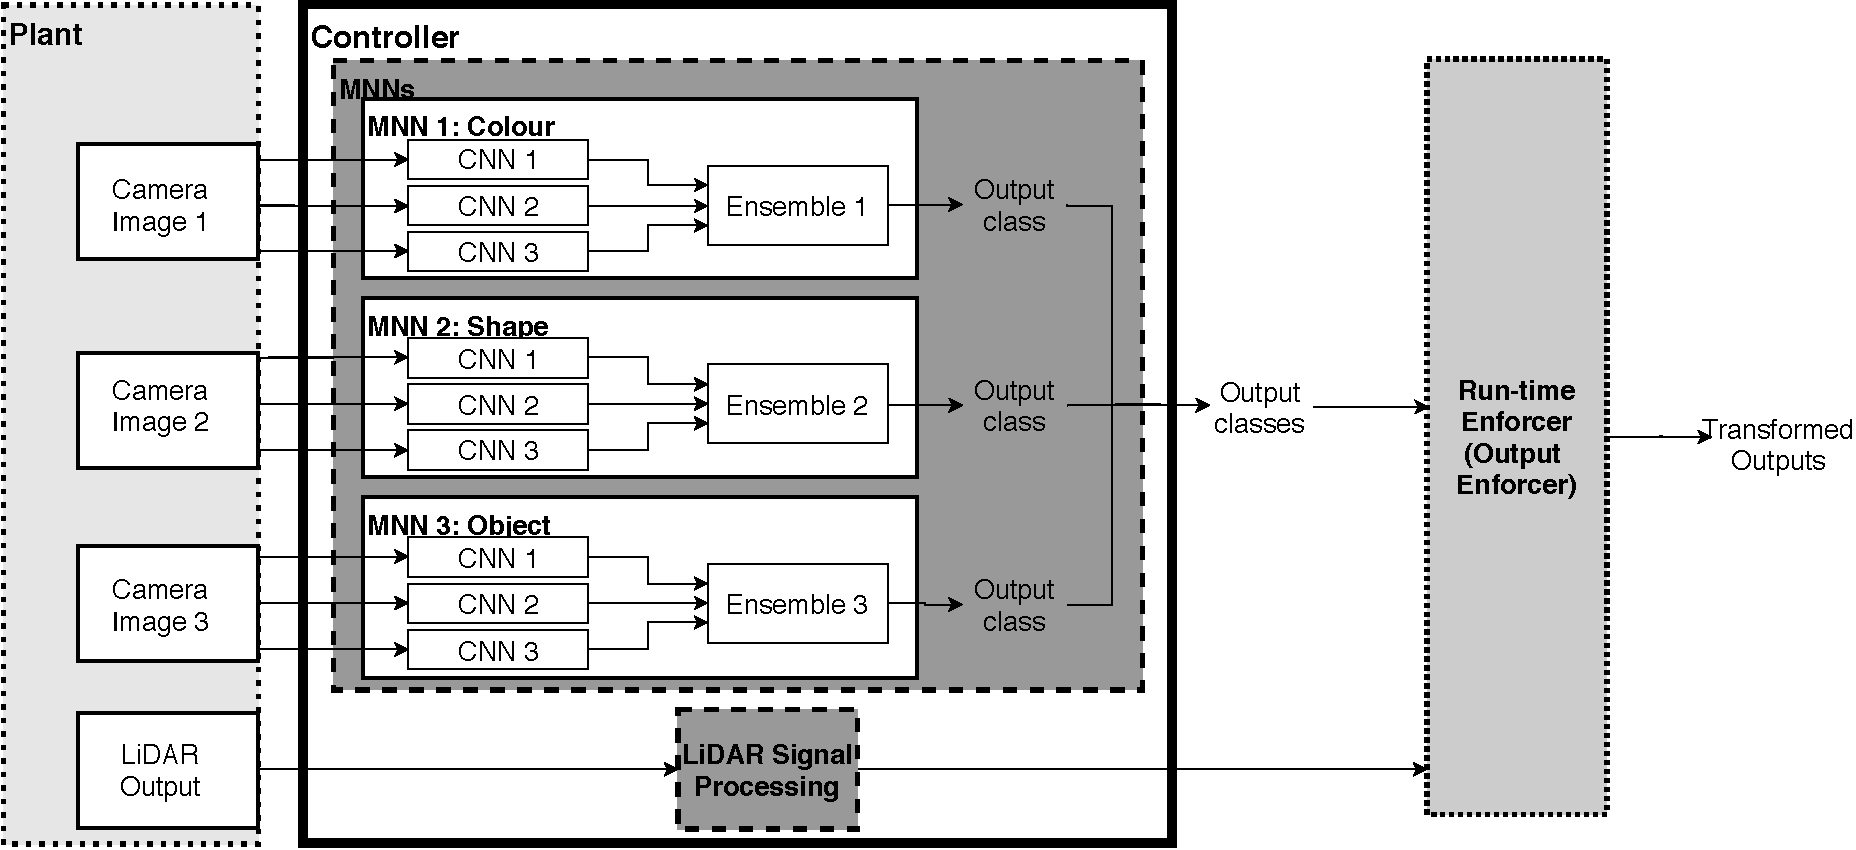
\includegraphics[width=\textwidth]{Content/fig/MNN.pdf}
	\caption{Block diagram showing the \acf{MNN} ensembles and run-time verifier used in this case study} \label{fig:mnn}
\end{figure}

Utilising synchronous semantics~\cite{benveniste2003synchronous}, a \acf{MNN}, containing three other \ac{MNN} ensembles, was created.
This structure can be seen in Figure~\ref{fig:mnn}.
A \ac{MNN} is a synchronous composition of multiple \acf{SNN}.
Each of the three \ac{MNN} ensembles were used to classify shape, colour and object type of each object being output by the camera.
Each ensemble synchronously combined the outputs of three different convolutional \acp{SNN}, providing increased prediction accuracy for shape, colour and object type. 
Each \ac{SNN} was implemented in the synchronous language Esterel~\cite{Esterel} using the Darknet library~\cite{darknet13} to train and implement the \ac{CNN}.
After the introduction of \acf{MNN2C}, this system was trained in Python using Keras~\cite{chollet2015keras} and converted to time-predictable \acp{SNN} in C.
These ensembles ran in synchronous concurrency with each other, forming a single, larger \ac{MNN}. 

The individual \ac{CNN} outputs were passed to an ensemble function that combined the classifications of each \ac{CNN} together, resulting in a more accurate overall classification.
Each ensemble used a custom averaging function that worked out the most likely class of the classified object using the top 2 most likely classes output by each \ac{CNN}.
The outputs of each ensemble were then combined into a batch of outputs forming the \textit{predicted output} for the colour, shape and object type of the detected object.

\subsection{Sensor Fusion for a Traffic Sign Recognition AV System}
Two sensors were used for the purpose of sensor fusion; \ac{LiDAR} and cameras.
The \ac{LiDAR} controller for this system used the 93\% accuracy of the research group in~\cite{lidarFusion}, to closely simulate a system using real \ac{LiDAR}.
The simulated camera outputs consisted of test images from both the \ac{VOC} 2012~\cite{pascal-voc-2012} and \ac{GTSRB}~\cite{Stallkamp2012-gtsrb} datasets, in a combination of people, vehicles and various traffic signs.
The \ac{LiDAR} and camera outputs were handled by different parts of the controller.
The camera outputs were fed into a \ac{MNN} (see Figure~\ref{fig:mnn}) where they were classified by shape, colour and object type.
Sensor fusion happened after classification occurred and was done by the run-time verifier.

\subsection{\acf{RV}~\cite{runtime-verify} for a Traffic Sign Recognition AV System}
The system controller was encapsulated by a run-time verifier~\cite{recps} that used sensor fusion to check for misclassifications made by the \ac{MNN}.
A run-time verifier gives a verdict on every I/O sequence given to it by the controller.
The \ac{RV} can be seen in Figure~\ref{fig:mnn}, between the controller and the plant, monitoring the outputs of the \ac{MNN} controller.
The run-time verifier was given a \acf{VDTA}, introduced in Chapter 4, as the safety policy to be used.
This \ac{VDTA} is shown in Figure~\ref{fig:signrte}.
The syntax for this figure is explained in Chapter 2.

\begin{figure}[h]
	\centering
	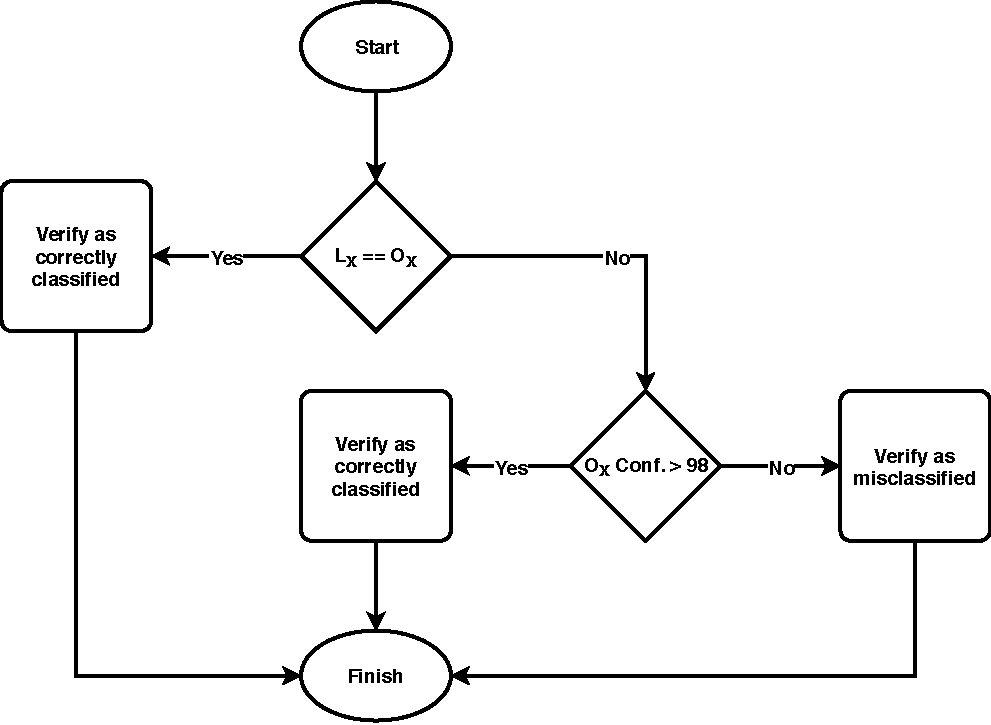
\includegraphics[width=\textwidth]{Content/fig/flow-misclassify.pdf}
	\caption{Flow-chart simplifying the algorithm used to detect misclassifications made by the \ac{MNN} controller.} \label{fig:flow}
\end{figure}

This policy uses a straight-forward algorithm to determine if an object has been misclassified or not.
For simplicity, this algorithm has been transferred to a flow-chart (Figure~\ref{fig:flow}), rather than being shown on the \ac{VDTA}.

\begin{figure}[h]
	\centering
	\scalebox{1}{

\begin{tikzpicture}[>=stealth',shorten >=1pt,auto,node distance=3 cm, scale = 1, transform shape]

\tikzstyle{accept} = [draw=blue!75,fill=blue!20]
\tikzstyle{violate} = [draw=red!75,fill=red!40, dashed]
\tikzstyle{unstable} = [draw=red!75,fill=red!15]

\node[initial,state, accepting, accept] (A) {$q_{auto}$};
\node[state, unstable] (B) [right of=A] {$q_{unstable}$};
\node[state, violate]         (C) [below of=B, xshift=-1.5cm]  {$q_v$};

\path[->] 
		(A) edge [loop above]       node [above]  
		{
			\scriptsize$\let\scriptstyle\textstyle\substack{\overline{M}}$
		} (A)
		
		(A) edge [bend left]		node [below]  
		{
			\scriptsize$\let\scriptstyle\textstyle\substack{
				M,~\\~
				t~:=~0~
			}$
		} (B)
	
		(B) edge [loop above]		node [above]  
		{
			\scriptsize$\let\scriptstyle\textstyle\substack{t~<~3~\&~\\~~\overline{M}}$
		} (B)
	
		(B) edge [bend left]		node [right]  
		{
			\scriptsize$\let\scriptstyle\textstyle\substack{M}$
		} (C)
	
		(B) edge [bend left]		node [below]  
		{
			\scriptsize$\let\scriptstyle\textstyle\substack{t~>=~3~\&\\~\overline{M}}$
		} (A)
	
		(C) edge [loop below] node [below]
		{
			\scriptsize$\sum$
		}(C)
		;

\end{tikzpicture}}
	\begin{itemize}
		\item $M$: Binary misclassification verdict: no misclassification (0) or misclassification detected (1).
		\item $t$: Timer for the unstable state.
	\end{itemize}
	
	\caption{Enforcer policy for the \acf{AV} prediction system}
	\label{fig:signrte}
\end{figure}

The automaton started in a safe state, where control of the vehicle was autonomously handled by the system controller.
If a misclassification was detected, the verified policy entered an unstable state, still under autonomous control. 
Once enough time passed without further misclassifications, the vehicle entered the safe state again.
However, if another misclassification was detected while unstable, the verified policy entered a violation state and control of the \ac{AV} was passed to the driver by the system.
The vehicle would not enter autonomous mode again until the system was restarted.






